\begin{frame}[title-small={color=hpiorange, bg=none, text=Implementation}]
	\maketitle
\end{frame}


\begin{frame}{Circuit Initialization - Classical Register (Bit-wise)}
  \begin{minipage}{1.0\textwidth}
    \begin{itemize}
      \item idea: describe classical state as bit string of length n and use register of $n$ qubits to represent as quantum state
      \item easy to implement, easy to measure
      \item limitations: large amount of qubits needed $\rightarrow$ hardware limitations, circuit complexity
      \item related works: [Corte2018] $\rightarrow$ reduce number of qubits, discard operations
    \end{itemize}
  \end{minipage}
\end{frame}


\begin{frame}{Circuit Initialization - State Purification}
  \begin{minipage}{1.0\textwidth}
    \begin{itemize}
      \item idea: describe a classical state as pure or mixed quantum state via density operation $\rho$
      \begin{itemize}
        \item pure state: $\rho = \Sigma_{i=1}^{n} |\psi\rangle \langle\psi |$, trace $Tr(\rho) = 1$
        \item mixed state: $\rho = \Sigma_{i=1}^{n} p_i |\psi_i\rangle \langle\psi_i |$, trace $Tr(\rho) < 1$
      \end{itemize}
      \item reduced density operation: two systems $A$ and $B$, then $\rho_{A} = Tr_B(\rho_{AB})$
      \begin{itemize}
        \item describe entangled states
        \item state purification: system $A$ in a mixed state $\rightarrow$ a composed system $AB$ can be found that complies with the reduced density operation $\rho_{A}$ and $AB$ in a pure state
      \end{itemize}
    \end{itemize}
  \end{minipage}
\end{frame}


\begin{frame}{Circuit Initialization - Amplitude Amplification}
  \begin{minipage}{0.5\textwidth}
    \begin{itemize}
      \item idea: "search" the quantum state via grover algorithm
      \begin{itemize}
        \item step 1: start in the uniform superposition $|s\rangle = H^{\otimes n}$
        \item step 2: apply oracle operation $U_f$
        \item step 3: apply reflection operation $U_s$, $U_s=2|s\rangle \langle s| -1$
      \end{itemize}
    \end{itemize}
  \end{minipage}%
  \hfill
  \begin{minipage}{0.5\textwidth}
    \centering
    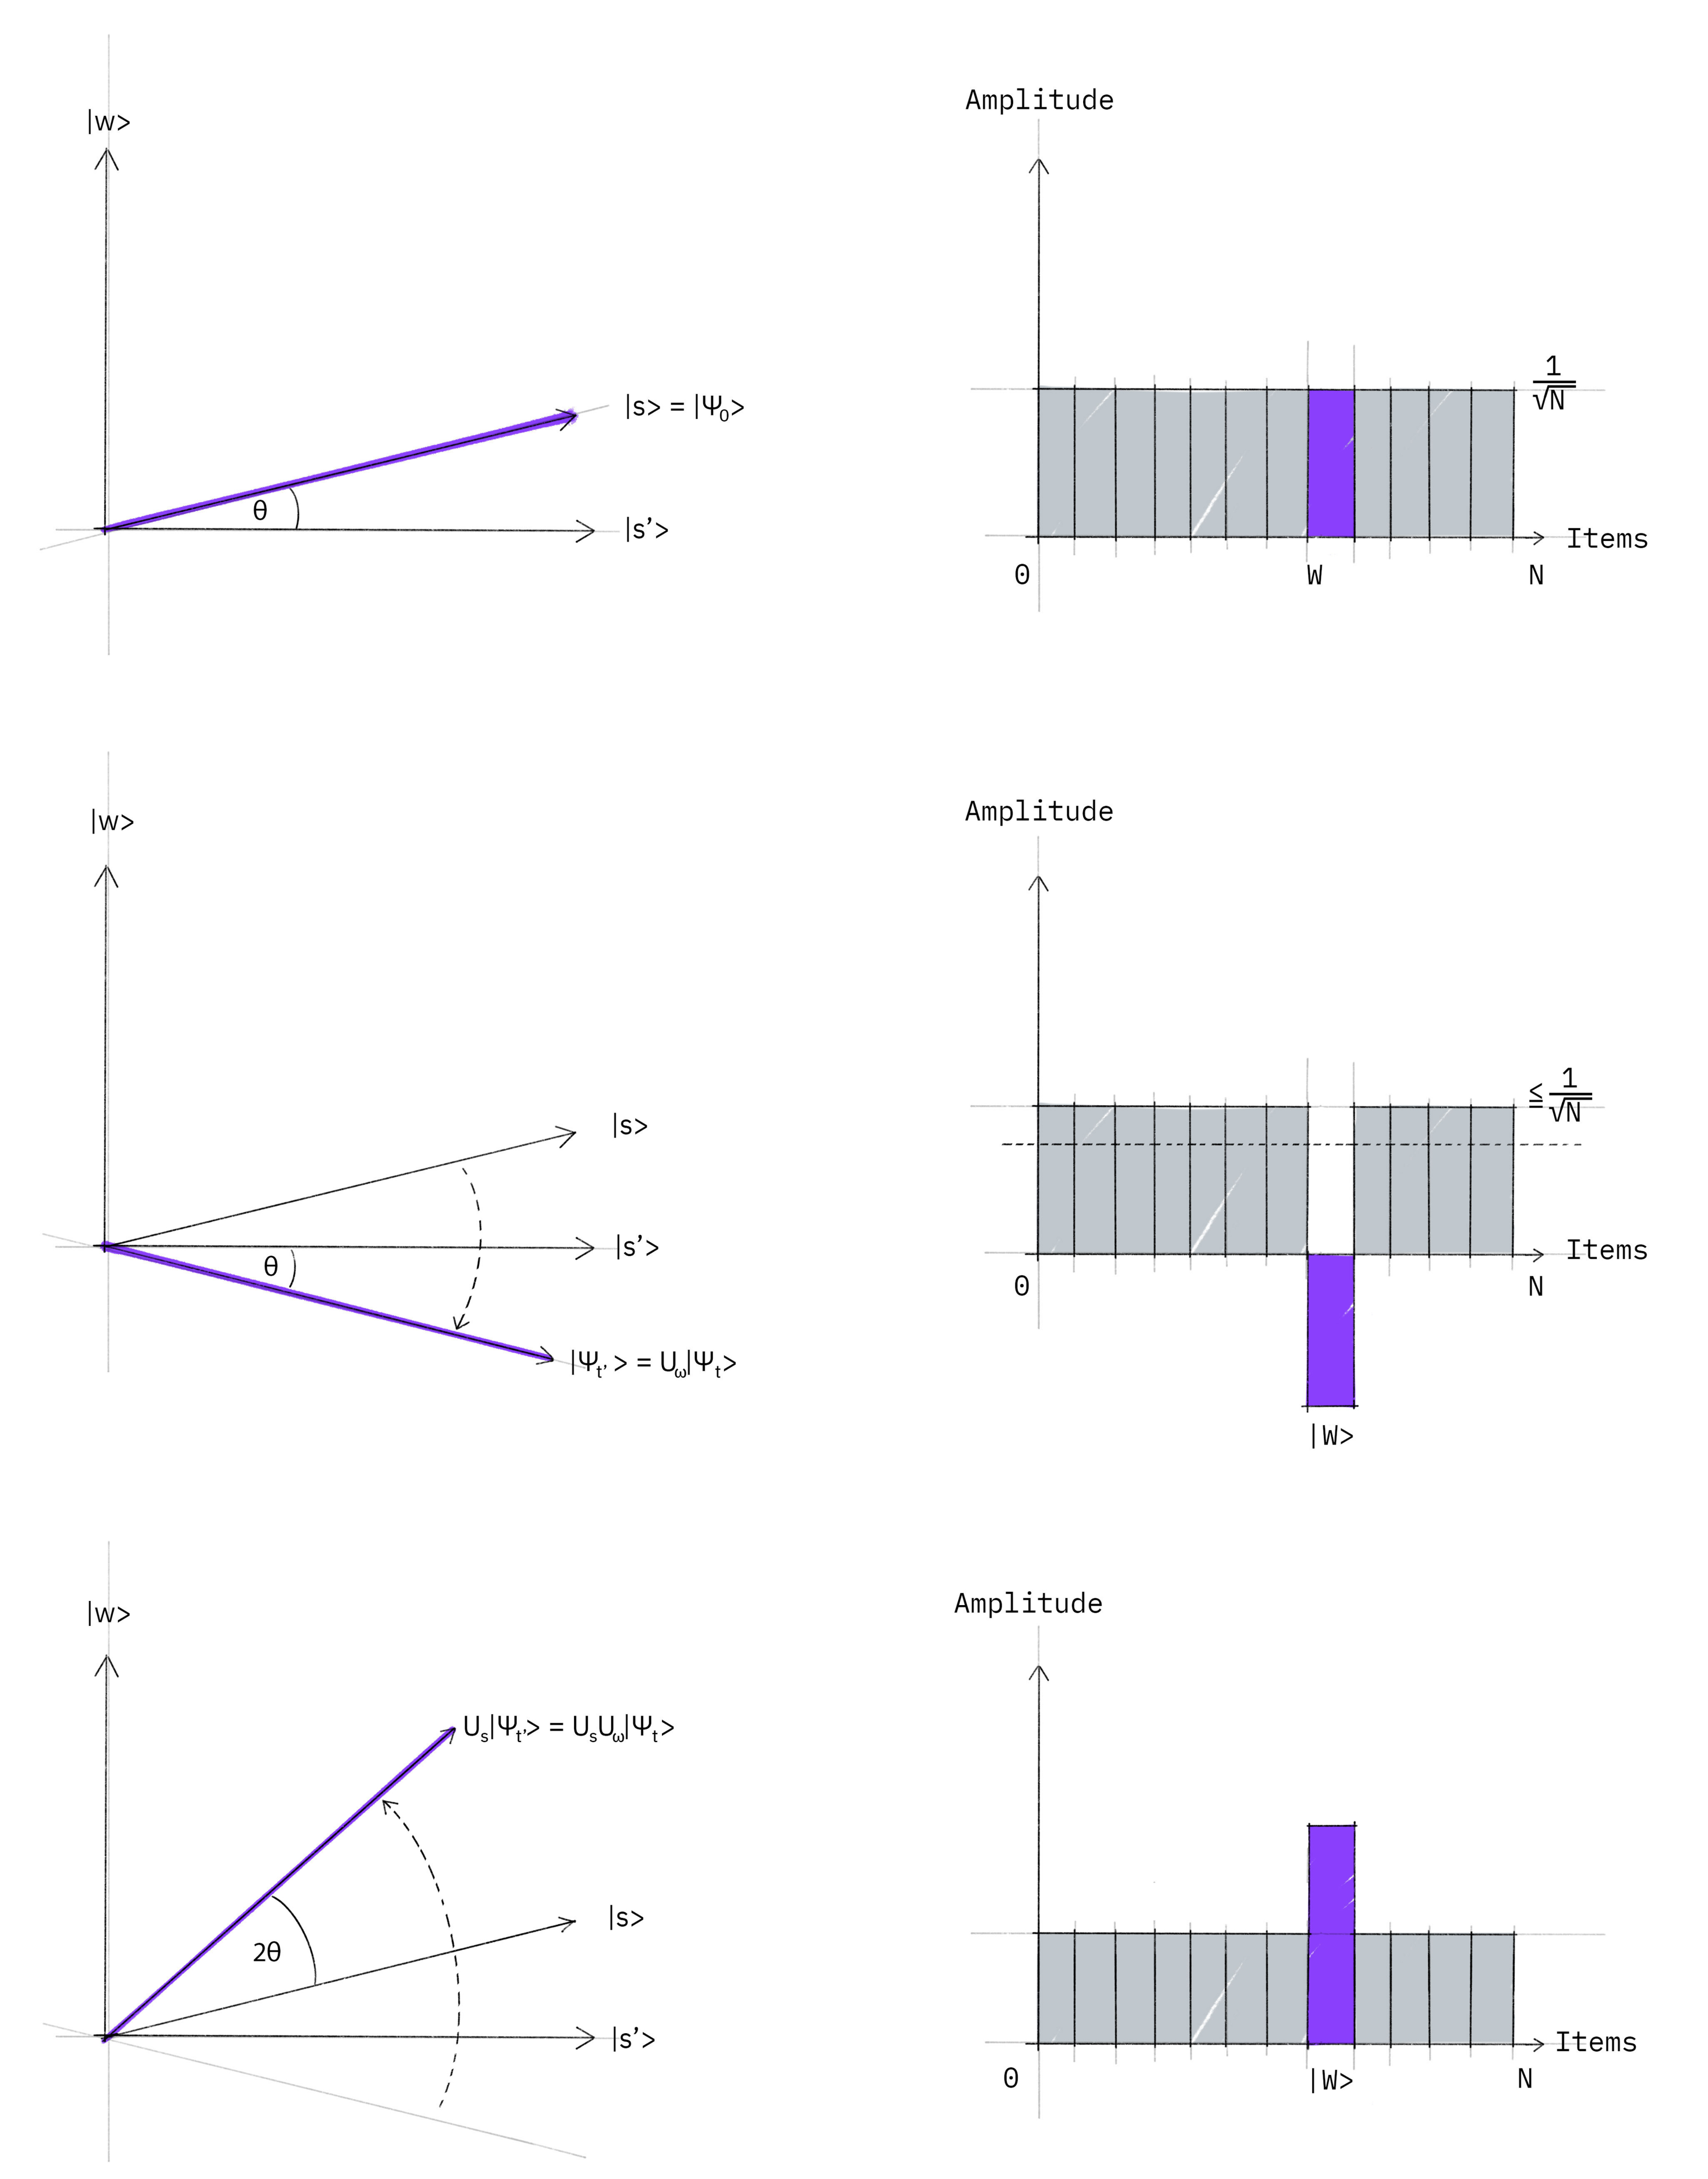
\includegraphics[width=0.8\textwidth]{../assets/grover_steps.png}
  \end{minipage}
  \footnote{\url{https://qiskit.org/textbook/ch-algorithms/grover.html}}
\end{frame}


\begin{frame}{Circuit Initialization ~ Challenges}
  \begin{minipage}{1.0\textwidth}
    \begin{itemize}
      \item textbook examples often quantum states that are easy to implement, e.~g. classical states
      \item paper examples often very brief description how to initialize quantum state
      \item method specifics:
      \begin{itemize}
        \item bit-wise: properly apply discard operations
        \item state purification: find composed state in respect to the density matrix of given data set
        \item amplitude amplification: find oracle operation in respect to the given data set
      \end{itemize}
    \end{itemize}
  \end{minipage}
\end{frame}


\begin{frame}{Simple Quantum PCA with Swap Test}
  \begin{minipage}{1.0\textwidth}
    \begin{itemize}
      \item used libraries: python, unittest, numpy, cirq
      \item cirq testing: package cirq.testing
      \begin{itemize}
        \item assert\_same\_circuits $\rightarrow$ tests if two circuits are \emph{equivalent} to each other
        \item assert\_has\_diagram $\rightarrow$ tests the text representation
      \end{itemize}
    \end{itemize}
  \end{minipage}
  \begin{minipage}{1.0\textwidth}
    \centering
    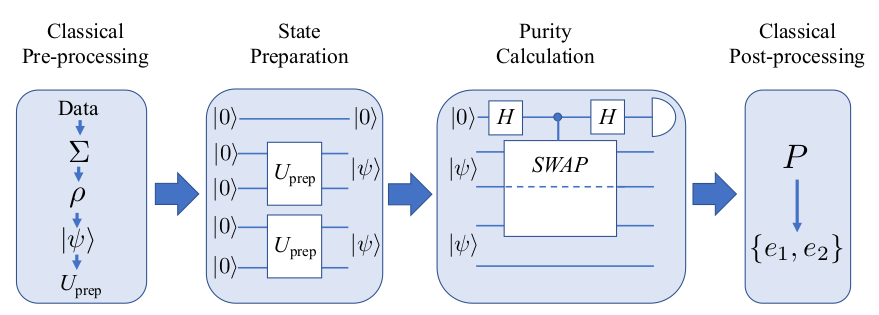
\includegraphics[width=0.8\textwidth]{../assets/context_algorithm_main-ref19.png}
  \end{minipage}
\end{frame}


\begin{frame}{Simple Quantum PCA with Swap Test - State Preparation}
  \begin{minipage}{0.5\textwidth}
    \begin{itemize}
      \item cirq: gate vs. operation vs. circuit
      \begin{itemize}
        \item implementation circuit initialization: internal method of "SimpleSwapTestQPCA" cirq circuit
        \item unitary preparation operation to initialize $|\psi\rangle$ can be computed independently
        \item circuit makes sure enough copies of $|\psi\rangle$ are initialized
      \end{itemize}
    \end{itemize}
  \end{minipage}%
  \begin{minipage}{0.5\textwidth}
    \begin{itemize}
      \item (code snippet here?)
    \end{itemize}
  \end{minipage}
\end{frame}


\begin{frame}{Simple Quantum PCA with Swap Test - Purify Calculation}
  \begin{minipage}{0.5\textwidth}
    \begin{itemize}
      \item swap test: operation to check level of difference of two quantum states
      \begin{itemize}
        \item input: two quantum states, each represented with $n$ qubits
        \item output: level of equality of the two states
      \end{itemize}
      \begin{itemize}
        \item if both states are orthogonal to each other: probability to measure $0$ is $\frac{1}{2}$
        \item if both states are equal to each other: probability to measure $0$ is $1$
      \end{itemize}
    \end{itemize}
  \end{minipage}%
  \begin{minipage}{0.5\textwidth}
    \centering
    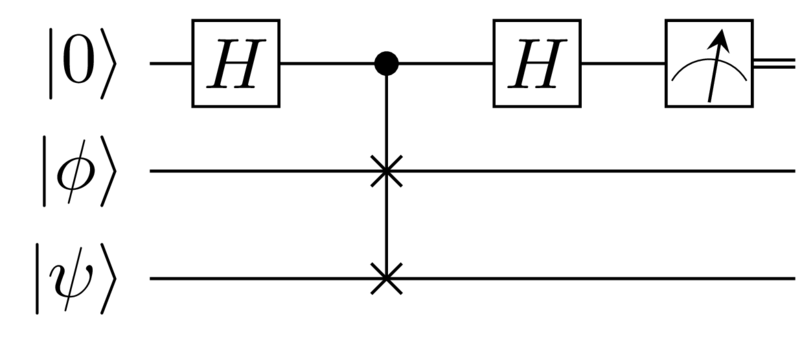
\includegraphics[width=0.8\textwidth]{../assets/wp_swap_test_simple.png}
  \end{minipage}
  \footnote{\url{https://en.wikipedia.org/wiki/Swap_test}}
\end{frame}


\begin{frame}{Simple Quantum PCA with Swap Test - Purify Calculation}
  \begin{minipage}{0.5\textwidth}
    \begin{itemize}
      \item cirq: gate vs. operation vs. circuit
      \begin{itemize}
        \item implementation swap test: cirq gate "SwapTestGate" and "swap test" function which returns a cirq operation
        \item drawback: gates only know qubits but not register of qubits $\rightarrow$ swap test composition makes some assumptions how qubits are entered into the gate
        \item better: directly implement as cirq operation
      \end{itemize}
      \item cirq: equality vs. value equality
      \item end-to-end testing: simulate circuit $\rightarrow$ find acceptable delta between expected and actual result
    \end{itemize}
  \end{minipage}%
  \begin{minipage}{0.5\textwidth}
    \begin{itemize}
      \item (code snipped swap test and swap test gate here?)
    \end{itemize}
  \end{minipage}
\end{frame}


\begin{frame}{Simple Quantum PCA with Swap Test - Post-processing}
  \begin{minipage}{1.0\textwidth}
    \begin{itemize}
      \item formula to calculate the two eigenvalues\footnote{[Lokho2020]} with purity $P = Tr(\rho^2)$:
      \begin{itemize}
        \item $e_1 = Tr(\Sigma) \ast (1 + \sqrt{1 - 2 (1 - P)}) / 2$
        \item $e_2 = Tr(\Sigma) \ast (1 - \sqrt{1 - 2 (1 - P)}) / 2$
      \end{itemize}
      \item this formula is specific for $2 \times 2$ matrices and maybe even mixed states
      \item example from [He2021]: formula does not calculate eigenvalues correctly 
    \end{itemize}
  \end{minipage}
\end{frame}


\begin{frame}{Enhancements with Quantum Phase Estimation}
  \begin{minipage}{1.0\textwidth}
    \centering
    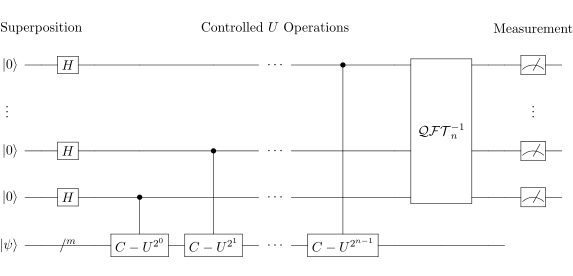
\includegraphics[width=0.7\textwidth]{../assets/wp_phase_estimation.png}
  \end{minipage}
  \footnote{\url{https://en.wikipedia.org/wiki/Quantum_phase_estimation_algorithm}}
  \begin{minipage}{1.0\textwidth}
    \begin{itemize}
      \item more generalized circuit for quantum based eigenvalue calculation
      \item algorithm can calculate $n$ eigenvalues not only two
      \item changes in the preprocessing: need to compute unitary operation for the QPE
      \item changes in the post-processing: calculate eigenvalues from amplitudes
    \end{itemize}
  \end{minipage}
\end{frame}
